\chapter{Compact Muon Solenoid}

\section{scratch}
Mention the location of CMS.  Give an overview of what it was designed to do.  Find a nice way to say that there is a lot of shit coming from the interaction region and we have to sort through it.  We need to get charged particle momentum and energy, electromagnetic energy, 

\section{Introduction}
About 100 meters below the town of Cessy, France at Point 5 is the Compact Muon Solenoid (CMS).  The CMS is a general purpose detector weighing 14,000 tonnes with a length of 28.7 meters and a 15.0-meter diameter.  A perspective view of of the detector is shown in Figure \ref{fig:cmsschematic}.
\begin{figure}[h]
	\centering
	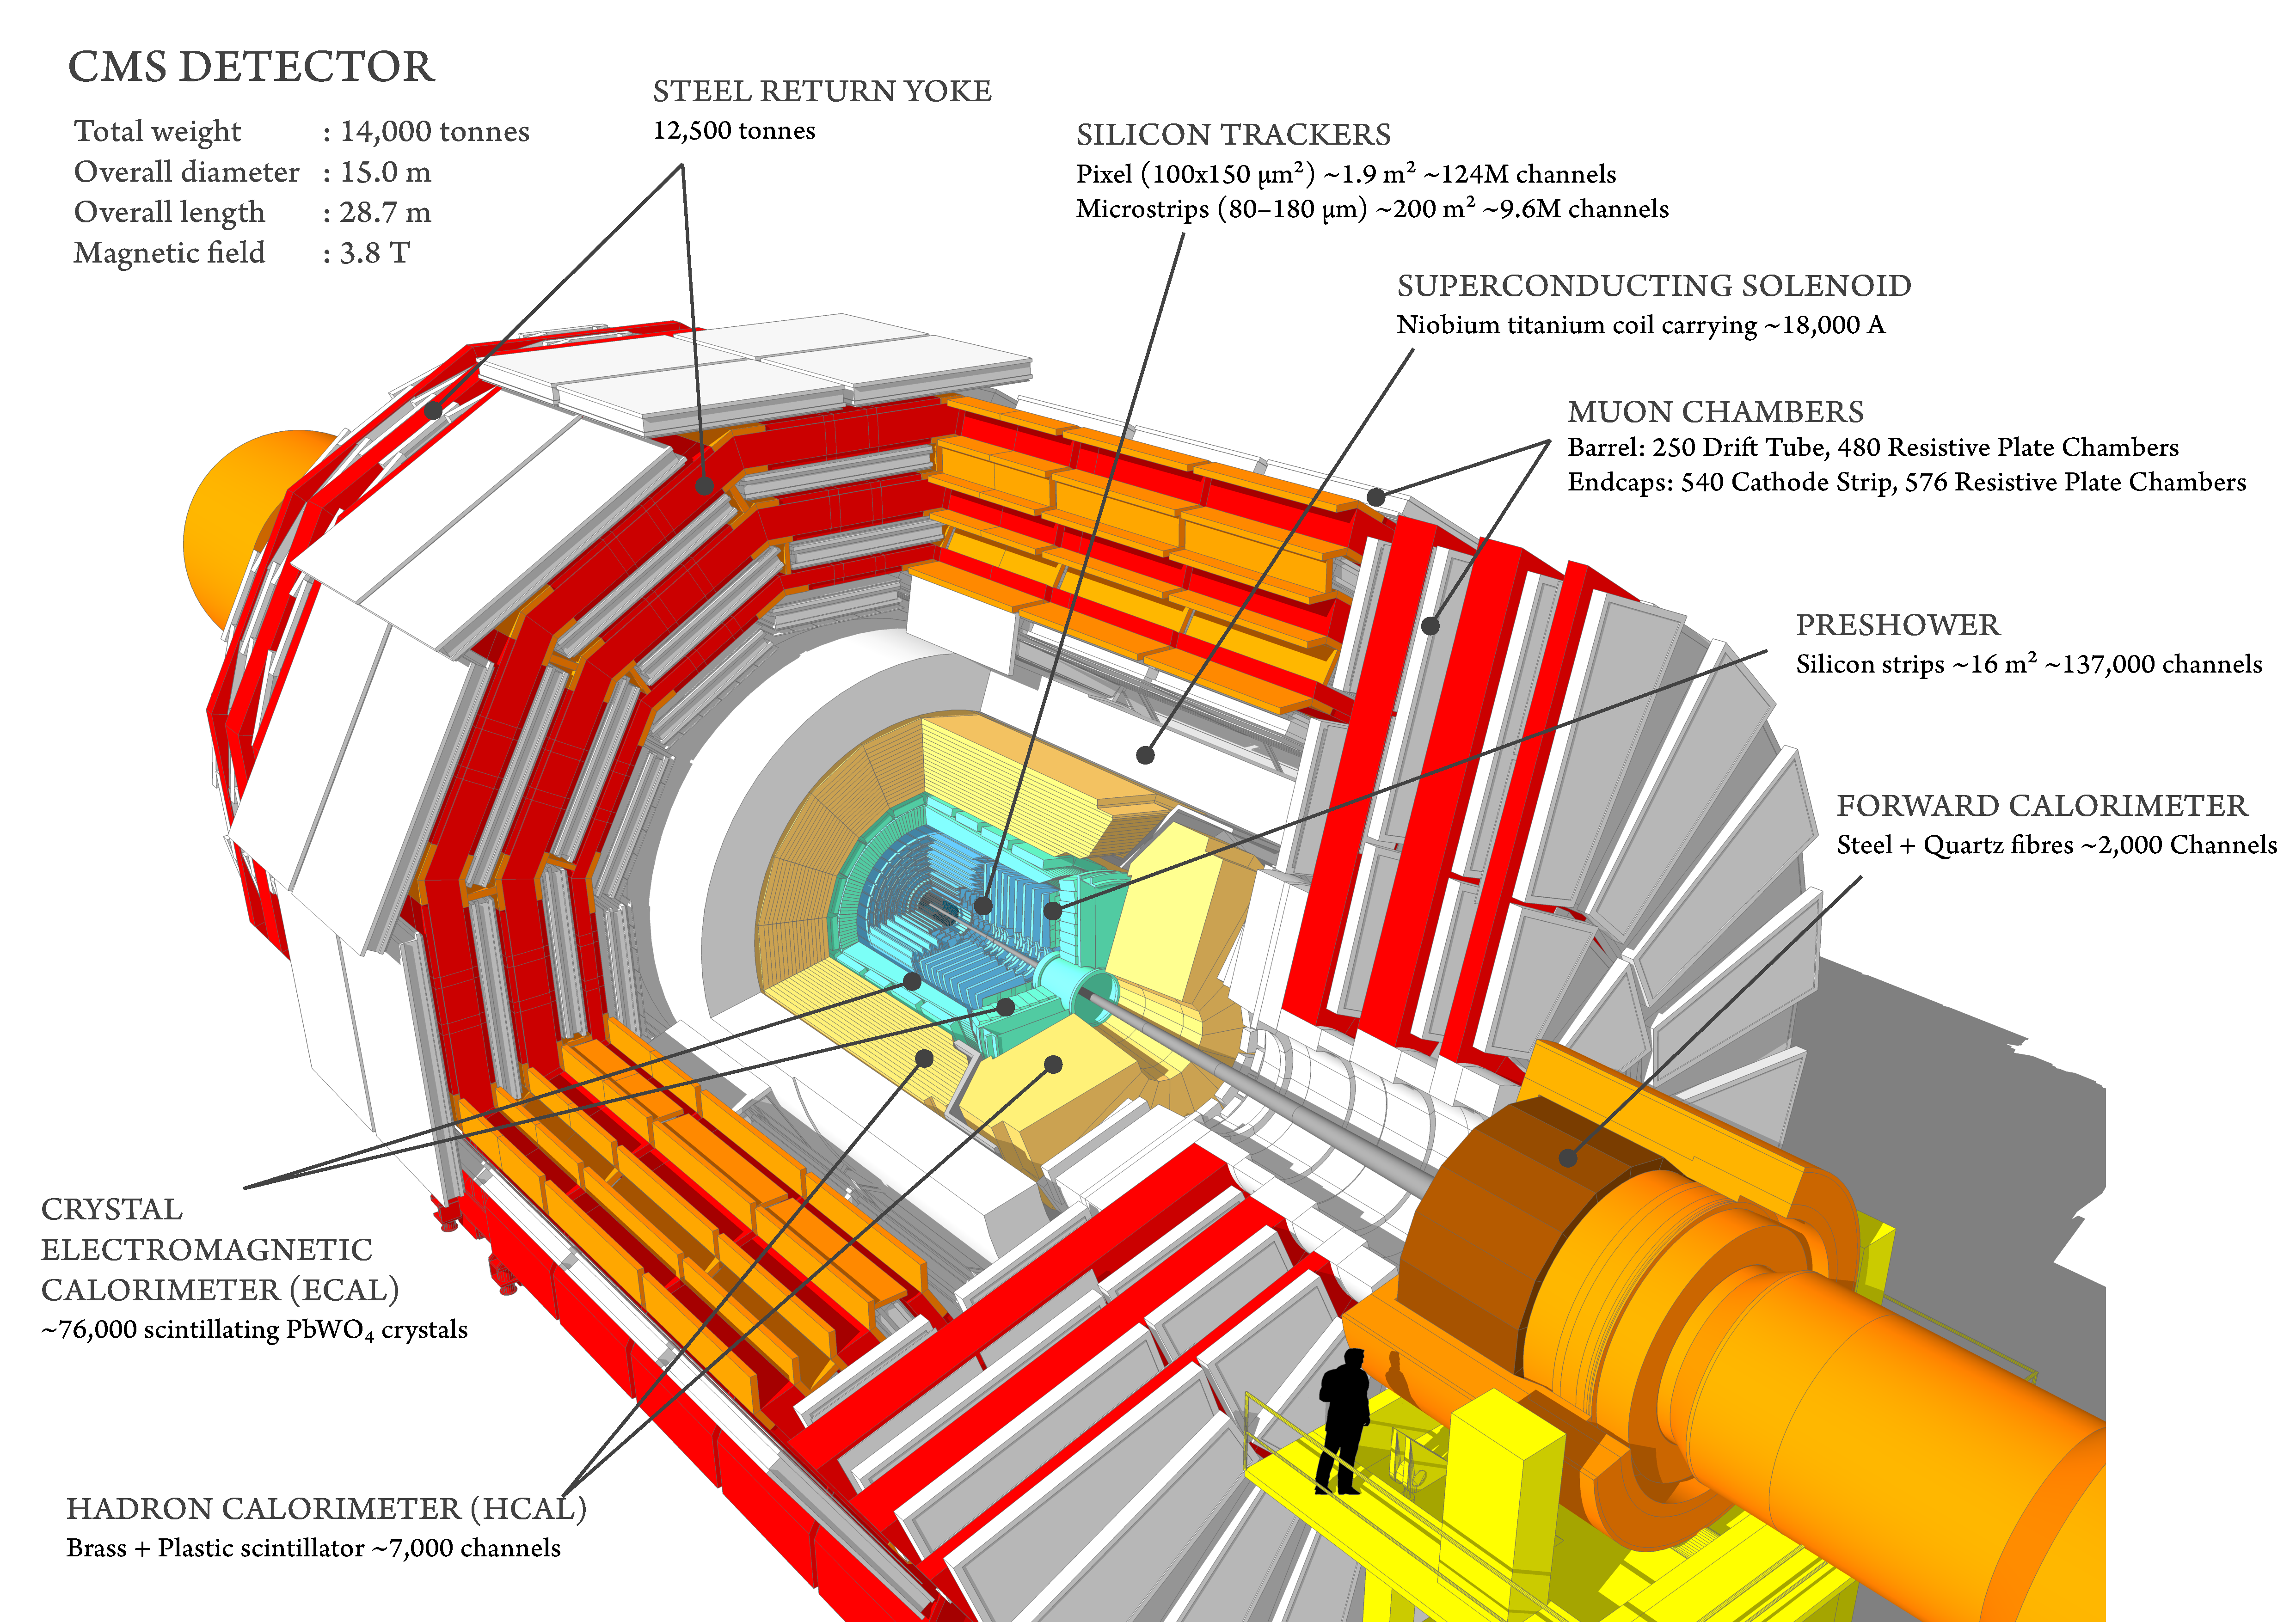
\includegraphics[width=0.7\linewidth]{Figures/cms_schematic}
	\caption{Schematic of CMS detector}
	\label{fig:cmsschematic}
\end{figure}


While the CMS detector was designed to study proton-proton collisions and heavy-ion collisions with center of mass energies up to 14 TeV and 5.5 TeV respectively, this document will focus on operating with proton-proton collisions. 

With a total proton-proton cross-section of about 300 mb at the LHC design energy of $\sqrt{s} = 14$ TeV one expects \cite{Collaboration_2008}.  At the LHC design luminosity of 10$^{34}$cm$^{-2}$s$^{-1}$